\section{Solving the multi-objective WSN problem}
\label{section:solution}
As defined in the previous Section, we seek a method to optimise multiple objectives in our WSN system. To do so we will incorporate two algorithms. We give the high-level purpose and requirements of each algorithm in the next sections, however, full details and theoretical justification can be found in \cite{creech2021dynamic, creech2021resource}.

\subsection{Optimisation algorithms for task allocation and resource allocation}
%%%%%%%%%%%%%%%%
\newcommand{\varAction}[2]{\varSymbol{a}{#1}{#2}}
\newcommand{\functionExec}[2]{\texttt{exec}(\varAtomicTask{}{})}
\newcommand{\functionAlloc}[2]{\texttt{alloc}(\varAtomicTask{}{}, \varAgent{}{})}
\newcommand{\functionInfo}[2]{\texttt{info}(\varAgent{}{})}
\newcommand{\functionLink}[2]{\texttt{link}(\varAgent{}{})}
\newcommand{\functionATARIA}[2]{
	\functionSignature{
		ataria_{\varAgent{}{}}
	}{
		\varAtomicTask{}{}, \varAgent{self}{}
	}
}	
\newcommand{\formalATARIA}[2]{
	\functionFormal{\texttt{ataria}_{\varAgent{}{}}}
	{\setAtomicTask{}{} \times \setAgents{}{}}
	{
	\texttt{exec}(\setAtomicTask{}{})
	\times \texttt{alloc}(\setAtomicTask{}{}, \setAgents{}{})
	\times \texttt{info}(\setAgents{}{})
	\times \texttt{link}(\setAgents{}{})
}
}
\newcommand{\functionMGRAO}[2]{\texttt{mgrao}(\varAtomicTask{}{}, \varAgent{self}{})}
\newcommand{\formalMGRAO}[2]{
	\functionFormal{\texttt{mgrao}_{\varAgent{}{}}}
	{\setAtomicTask{}{} \times \setRealNumbers{}{}}
	{
		\setRealNumbers{}{}
	}
}
\newcommand{\functionMGRAOUpdate}[2]{
	\texttt{mgrao-update}_{\varAgent{}{}}
	(\varAtomicTask{}{}, \functionTaskAbsoluteValue{}{})}
%%%%%%%%%%%%
	
The \acronymATARIAExtended{}{} algorithm enables agents in the system to learn the best actions to take given their current state. This ranges from deciding which other agents to allocate tasks to and obtain the best composite task values, to exploring the system for other agents, and adapting connectivity to handle network disruption. An agent uses the \acronymATARIA{}{} algorithm to choose an action to take, which can be one of the following,
\begin{enumerate}
	\item $\functionExec{}{}$, The agent will execute the atomic task $\varAtomicTask{}{}$ itself.
	\item $\functionAlloc{}{}$, the agent will allocate the atomic task $\varAtomicTask{}{}$ to another agent $\varAgent{}{}$.
	\item $\functionInfo{}{}$, the agent will request information from another agent $\varAgent{}{}$.
	\item $\functionLink{}{}$, the agent will allocate resources to hold information on the agent $\varAgent{}{}$ and maintain a connection.
\end{enumerate}
The \acronymATARIA{}{} algorithm learns to select the actions that generate the best composite task values, and adapt the choice of action depending on how good the composite task values are in comparison to the historical values through the updating of Q-values in its temporal-update algorithm. The algorithm will select one of the possible actions for the agent $\varAgent{}{}$, given it has non-completed, allocated tasks $\setAtomicTask{}{}$, and knows of other agents $\setAgents{}{}$. $\label{eq:ataria}\formalATARIA{}{}$.
The \acronymMGRAOExtended{}{} algorithm helps agents executing measurement tasks allocate their resources to optimise the composite task value as well. This has two parts, an update algorithm that adjust weights of resources based on received atomic task values, and the application of these weights to generate the task execution quality itself. The update algorithm will update the resource weightings for an agent, given the type of an atomic task it completed, and the absolute task value of that task to another agents' composite task, $\label{eq:mgrao}\formalMGRAO{}{}$.



\subsection{Extension to hierarchical task allocation}

To enable agents to form arcs as described we allow atomic tasks to be re-allocated to further agents in order to reach an agent within range of a demand point. Figure \ref{fig:arc-flow} illustrates an arc where there are two re-allocations needed before a specific atomic task is allocated to an agent whose sensor is in range of the demand point, and can therefore make a measurement.

\begin{figure}[ht]
	\centering
	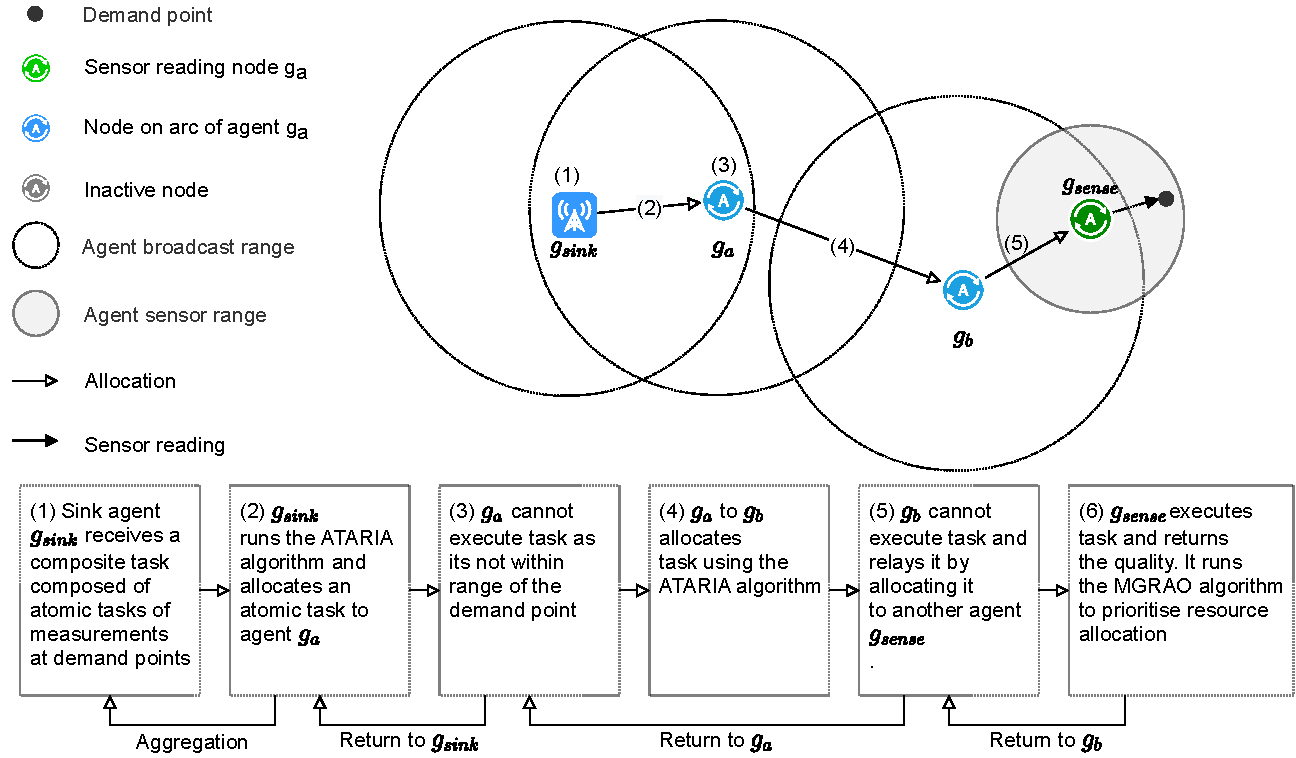
\includegraphics[width=0.8\linewidth, trim={25pt 0pt 25pt 0pt, clip}]{arc-flow}
	\caption{\textbf{Allocation along an arc}. This diagram illustrates how allocations can be relayed along an arc using successive applications of the \acronymATARIA{}{} algorithm.}
	\label{fig:arc-flow}
\end{figure}

